\chapter{变化的电磁场}

\begin{introduction}
	\item \nameref{9.1}
	\item \nameref{9.2}
	\item \nameref{9.3}
	\item \nameref{9.4}
	\item \nameref{9.5}
	\item \nameref{9.6}
\end{introduction}

\section{电磁感应的基本定律}\label{9.1}

$\bullet$ \textbf{电磁感应现象}

回路中产生的电流为感应电流, 而驱动电流的电动势则称为感应电动势. 

$\bullet$ \textbf{楞次定律}

\begin{axiom}[楞次定律]
	闭合回路中感应电流的方向, 总是使得这个电流在回路中所产生的磁通量, 去补偿或反抗引起感应电流磁通量的变化.
\end{axiom}

$\bullet$ \textbf{法拉第电磁感应定律}

\begin{axiom}[法拉第电磁感应定律]
	不论何种原因, 使通过回路所包围的面积的磁通量发生变化时, 回路中产生的感应电动势的大小与穿过回路的磁通量对时间的变化率成正比. 
	
	在国际单位制中, 有
	
	\begin{equation}
		\mathscr{E} = - \dv{\varPhi}{t} \label{C9-eq1}
	\end{equation}
	
	$\mathscr{E}$, $\varPhi$, $t$单位分别为V(伏特), Wb(韦伯), s(秒). 
	
	负号表明了感应电动势的方向, 说明感应电动势所产生的感应电流在回路中产生的磁通量总是反抗引起感应电流磁通量的变化. 
\end{axiom}

若闭合回路是由$n$匝线圈串联而成的, 那么当线圈的磁通量变化时, 每匝线圈中都将产生感应电动势, 显然在整个线圈中产生的感应电动势是每匝线圈中产生的感应电动势之和, 即

\begin{equation}
	\mathscr{E} = - \qty(\dv{\varPhi_1}{t} + \dv{\varPhi_2}{t} + \cdots + \dv{\varPhi_N}{t}) = - \dv{t} \qty(\sum\limits_{i = 1}^{N} \varPhi_i) = - \dv{\varPsi}{t} \label{C9-eq2}
\end{equation}

这里$\varPsi = \sum\limits_{i = 1}^{N} \varPhi_i$为穿过各匝线圈磁通量的总和, 称为穿过线圈的磁通链数, 简称磁链. 

若各匝线圈的磁通量相等均为$\varPhi$, 则$N$匝线圈的磁链

\begin{equation}
	\varPsi = N \varPhi \label{C9-eq3}
\end{equation}

此时

\begin{equation}
	\mathscr{E} = -\dv{\varPsi}{t} = -N\dv{\varPhi}{t} \label{C9-eq4}
\end{equation}

\section{动生电动势和感生电动势}\label{9.2}

\subsection{动生电动势}

\begin{figure}[H]
	\centering
	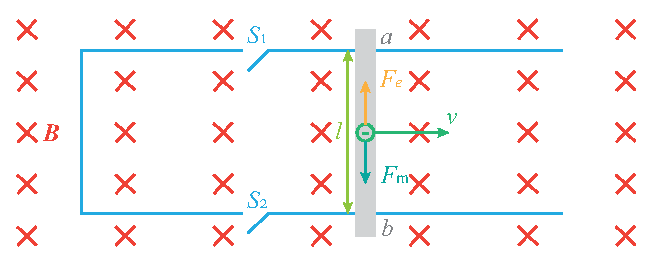
\includegraphics[scale=0.9]{C9-fig1.eps}
\end{figure}

设长为$l$的导体棒的自由电子将随棒仪器以速度$\va*{v}$在磁场中运动, 都受到洛伦兹力$\va*{F}_{\textrm{m}}$的作用

\begin{equation*}
	\va*{F}_{\textrm{m}} = -e \va*{v} \times \va*{B}
\end{equation*}

其中, $-e$为电子所带的电荷, 洛伦兹力$\va*{F}_{\textrm{m}}$方向从$a$指向$b$, 在$\va*{F}_{\textrm{m}}$作用下, 自由电子沿棒向下运动. 

若图中$S_1$, $S_2$闭合, 回路中将形成$a \to d \to c \to b \to a$的逆时针方向的电流; 若$S_1$, $S_2$断开, 自由电子运动的结果是使两端$ab$出现上正下负的电荷堆积, 从而产生自$a$指向$b$的静电场$\va*{E}$, 这样电子会受到一个与洛伦兹力方向相反的静电力$\va*{F}_e = - e \va*{E}$. 

在$\va*{F}_{\textrm{m}}$作用下, 自由电荷在两端堆积, $\va*{F}_e$越来越大, 当$F_{\textrm{m}} = F_e$时, 自由电子不再做定向运动, 此时非静电力为洛伦兹力, 非静电场的场强$\va*{E}_{\text{非}}$就是作用在单位正电荷上的洛伦兹力. 

\begin{equation}
	\va*{E}_{\text{非}} = \dfrac{\va*{F}_{\text{非}}}{e} = \va*{v} \times \va*{B} \label{C9-eq5}
\end{equation}

棒$ab$上的电动势为

\begin{equation}
	\mathscr{E} = \int_{-}^{+} \va*{E}_{\text{非}} \dd{\va*{l}} = \int_{a}^{b} \qty(\va*{v} \times \va*{B}) \dd{\va*{l}} \label{C9-eq6}
\end{equation}

一般情况下, 对于任意形状的一段导线$ab$, 在恒定的非均匀磁场任意运动或形变时, $\dd{\va*{l}}$线元的电动势为

\begin{equation*}
	\dd{\mathscr{E}} = \va*{E}_{\text{非}} \cdot \dd{\va*{l}} = \qty(\va*{v} \times \va*{B}) \dd{\va*{l}}
\end{equation*}

总电动势为所有线元电动势之和, 即

\begin{equation}
	\mathscr{E} = \int_{L} \dd{\mathscr{E}} = \int_{L} \qty(\va*{v} \times \va*{B}) \cdot \dd{\va*{l}} \label{C9-eq7}
\end{equation}

\begin{note}
	
	判断电势高低的方法
	
	(1) 方法一: 
	
	由$\mathscr{E} = \int_{a}^{b} \qty(\va*{v} \times \va*{B}) \cdot \dd{\va*{l}}$求出, 说明积分路径$b \to a$是沿着非静电场$\va*{E}_{\text{非}}$方向进行的. 
	
	故, 若$\mathscr{E} > 0$, 则$\varphi_a > \varphi_b$; 若$\mathscr{E} < 0$, 则$\varphi_a < \varphi_b$. 
	
	对图()中棒$ab$的电动势, 由于$\va*{v}$, $\va*{B}$, $\dd{\va*{l}}$三者相互垂直, 则有
	
	\begin{equation}
		\mathscr{E}_{ab} = \int_{a}^{b} \qty(\va*{v} \times \va*{B}) \cdot \dd{\va*{l}} = \int_{a}^{b} vB \dd{l} = BVl \label{C9-eq8}
	\end{equation}
	
	上式为棒在均匀磁场中动生电动势通式. 
	
	(2) 方法二: 
	
	在电流内部, 非静电场场强的指向是指向电源正极极板的, 动生电动势中, 非静电场场强$\va*{E}_{\text{非}} = \va*{v} \times \va*{B}$.
	
	由此可得, 由右手定则判断得$\va*{v} \times \va*{B}$得大拇指指向就是电势高的一端. 
	
\end{note}

\textbf{洛伦兹力一方面接受外力的功: 另一方面同时驱动电荷运动做功, 它不提供能量, 而只是传递能量, 起到能量转化的作用. }

\begin{example}
	如图所示, 长度为$L$的金属棒在垂直于均匀磁场$\va*{B}$的平面内沿逆时针绕$O$点匀速转动, 角速度为$\omega$, 求: 
	(1) 金属棒中感应电动势的大小和方向, OA间的电势差; 
	(2) 如果把金属棒改为半径为L的金属圆盘, 试求盘心和盘边缘之间的电势差. 
	
	\begin{figure}[H]
		\centering
		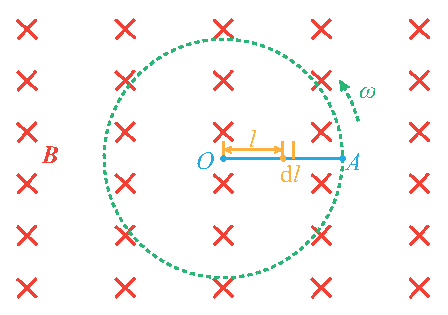
\includegraphics[scale=1.0]{C9-fig2.eps}
	\end{figure}
	
	\begin{solution}
		
		(1) 方法一: 用动生电动势求解
		
		在金属棒上任取有向元段$\dd{\va*{l}}$, 由于$\va*{v}$与$\va*{B}$垂直, 且$\va*{v} \times \va*{B}$与$\dd{\va*{l}}$反向, 则
		
		\begin{equation*}
			\dd{\mathscr{E}} = \qty(\va*{v} \times \va*{B}) \cdot \dd{\va*{l}} = vB\sin \dfrac{\pi}{2} \dd{l} \cdot \cos \pi = -vB \dd{l}
		\end{equation*}
		
		又
		
		\begin{equation*}
			v = \omega l
		\end{equation*}
		
		则
		
		\begin{equation*}
			\dd{\mathscr{E}} = -\omega B l \dd{l}
		\end{equation*}
		
		进一步
		
		\begin{equation*}
			\mathscr{E}_{AO} = \int_{O}^{A} \dd{\mathscr{E}} = - \int_{0}^{l} \omega B l \dd{l} = - \dfrac{1}{2} B \omega L^2
		\end{equation*}
		
		负号表示电动势从$A$指向$O$, 即$O$的电势比点高.
		
		故
		
		\begin{equation*}
			U_{OA} = \dfrac{1}{2} B \omega L^2
		\end{equation*}
		
		方法二: 用法拉第电磁感应定律求解
		
		设棒$OA$在时间$\dd{t}$内转过$\dd{\theta}$, 它扫过的面积为$\dd{S}$, 显然有
		
		\begin{equation*}
			\dd{S} = \dfrac{1}{2} L^2 \dd{\theta}
		\end{equation*}
		
		通过此面积的磁通量为
		
		\begin{equation*}
			\dd{\varPhi} = \va*{B} \dd{\va*{S}} = \dfrac{1}{2} B L^2 \dd{\theta}
		\end{equation*}
		
		由法拉第电磁感应定律, 得
		
		\begin{equation*}
			\abs{\mathscr{E}} = \abs{-\dv{\varPhi}{t}} = \dfrac{1}{2} B L^2 \dv{\theta}{t} = \dfrac{1}{2} B \omega L^2
		\end{equation*}
		
		(2) 若把金属棒换成金属盘, 可以把金属盘想象成无数根并联的金属棒$OA$组合而成. 因为金属棒是并联, 所以盘中心与边缘之间电势差为$U_{OA}$的值. 
		
	\end{solution}
	
\end{example}

\begin{example}
	导线$L$以角速度$\omega$绕其一固定端$O$, 在竖直长电流$I$所在平面内旋转, $O$点至电流$I$的距离为$a$, 且$a>L$, 如图所示. 求导线$L$在与水平方向成$\theta$角时动生电动势的大小和方向. 
	
	\begin{figure}[H]
		\centering
		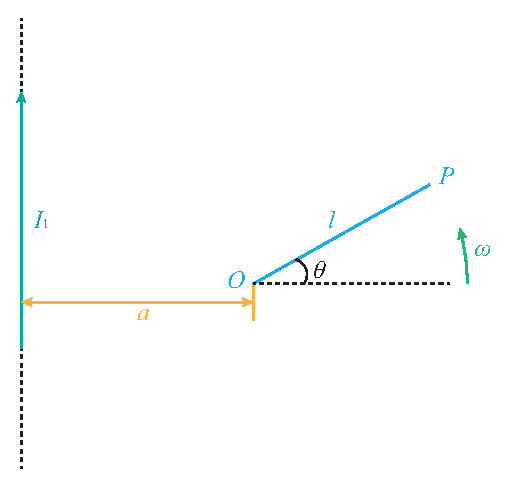
\includegraphics[scale=0.7]{C9-fig3.eps}
	\end{figure}
	
	\begin{solution}
		
		按照动生电动势计算公式, 可知
		
		\begin{equation*}
			\mathscr{E} = \int_{0}^{l} \qty(\va*{v} \times \va*{B}) \cdot \dd{\va*{l}} = - \int_{0}^{l} vB \dd{l} = - \int_{0}^{l} \omega l \dfrac{\mu_0 I}{2 \pi \qty(a + l \cos \theta)} \dd{l}
		\end{equation*}
		
		令
		
		\begin{equation*}
			x = a + l \cos\theta \Rightarrow \dd{l} = \dfrac{\dd{x}}{\cos \theta}
		\end{equation*}
		
		则
		
		\begin{align*}
			\mathscr{E} &= - \dfrac{\omega \mu_0 I}{2 \pi} \int_{a}^{a+L\cos\theta} \dfrac{x-a}{x\cos\theta} \dfrac{\dd{x}}{\cos \theta} \\
			&= \dfrac{\omega \mu_0 I}{2 \pi \cos^2 \theta} \int_{a}^{a+L\cos\theta} \qty(\dfrac{a}{x} - 1) \dd{x} \\
			&= \dfrac{\omega \mu_0 I}{2 \pi \cos^2 \theta} \qty(a \ln 
			\dfrac{a+L\cos\theta}{a} - L \cos\theta)
		\end{align*}
		
		电动势方向由$P$指向$O$, 即$O$点电势高. 
		
	\end{solution}
	
\end{example}

由上面的粒子可得, 计算动生电动势的基本方法: 

\begin{enumerate}[itemindent=1em]
	
	\item 由电动势定义求解
	
	\begin{equation*}
		\mathscr{E} = \oint_{L} \va*{E}_{\text{非}} \cdot \dd{\va*{l}} = \oint_{L} \qty(\va*{v} \times \va*{B}) \cdot \dd{\va*{l}}
	\end{equation*}
	
	若动生电动势仅在回路的一部分中产生, 则
	
	\begin{equation*}
		\mathscr{E} = \underset{\left( \text{经过内电路} \right)}{\int_{-}^{+}} \left( \va*{v} \times \va*{B} \right) \cdot \dd{\va*{l}}
	\end{equation*}
	
	经过内电路问题. 
	
	\item 由法拉第电磁感应定律求解
	
	\begin{equation*}
		\mathscr{E} = - \dv{\varPhi}{t} ~\text{或}~ \mathscr{E} = - \dv{\varPsi}{t}
	\end{equation*}
	
	有两种情况: 
	
	\begin{enumerate}[itemindent=1em]
		
		\item 闭合导线回路的整体或局部在磁场中运动. 这时先求出任意时刻$t$通过回路的磁链$\varPsi(t)$, 然后求出$\dv{\varPsi(t)}{t}$得到电动势的大小, 电动势的方向求楞次定律判断. 
		
		\item 一段不闭合导线在磁场中运动. 可假想构成一个闭合回路, 通常令假想部分不动, 因而不产生电动势, 这样, 由法拉第定律求出的回路所产生的感应电动势便是运动导线产生的电动势. 或先求出运动导线在$\dd{t}$时间内扫过面积的磁通量$\dd{\varPhi}$, 然后由$\dv{\varPhi}{t}$得到运动导线的动生电动势. 
		
	\end{enumerate}
	
\end{enumerate}

\subsection{感生电动势}

不管是否存在导体或导体回路, 随着时间变化的磁场, 总要在其周围空间激发电场, 这种电场叫\textbf{感生电场}. 

感生电场具有涡旋性, 它的电场线是无头无尾的涡旋状闭合曲线, 因此, 感生电场又称为涡旋电场或有旋电场. 

\begin{equation}
	\oint_{S} \va*{E}_{\text{感}} \dd{\va*{S}} = 0 \label{C9-eq9}
\end{equation}

这就是感生电场的高斯定理, 说明\textbf{感生电场是无源场}. 

计算感生电动势的基本方法: 

\begin{enumerate}[itemindent=1em]
	
	\item 由电动势的定义求解
	
	当导体回路闭合时, 感生电动势可写成
	
	\begin{equation}
		\mathscr{E} = \oint_{L} \va*{E}_{\text{感}} \cdot \dd{\va*{l}} \label{C9-eq10}
	\end{equation}
	
	当导体回路不是闭合回路时, 则
	
	\begin{equation}
		\mathscr{E} = \int_{L} \va*{E}_{\text{感}} \cdot \dd{\va*{l}} \label{C9-eq11}
	\end{equation}
	
	这种方法仅用于感生电场强度$\va*{E}_{\text{感}}$已知或容易求出的情况. 
	
	\item 由法拉第电磁感应定律求解
	
	\begin{equation}
		\mathscr{E} = -\dv{\varPhi}{t} = - \int_{S} \pdv{\va*{B}}{t} \dd{\va*{S}} \label{C9-eq12}
	\end{equation}
	
	用这种方法求解时, 导体回路必须闭合, 如果不闭合, 则要用辅助线构成闭合回路. 
	
\end{enumerate}

\begin{example}
	如图所示, 一电荷线密度为$\lambda$的长直带电线$l$与一正方形共面并与其一对边平行, 以变速率$v = v(t)$沿着其长度方向运动, 正方形线圈中的总电阻为$R$, 求$t$时刻方形线圈中感应电流$i(t)$的大小(不计线圈本身的自感).
	
	\begin{figure}[H]
		\centering
		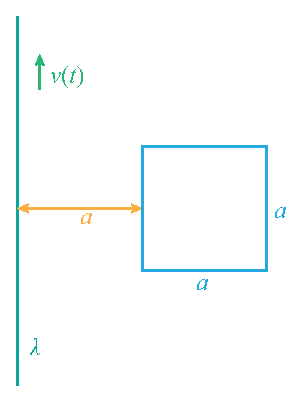
\includegraphics[scale=1.0]{C9-fig4.eps}
	\end{figure}
	
	\begin{solution}
		
		长直带电线运动相当于电流: 
		
		\begin{equation*}
			I = \dv{q}{t} = \lambda \dv{l}{t} = \lambda v
		\end{equation*}
				
		正方形圈内的磁通量
		
		\begin{equation*}
			\varPhi = \int \dd{\varPhi} = \int_{0}^{a} \dfrac{\mu_0}{2 \pi} \dfrac{I a}{a+x} \dd{x} = \dfrac{\mu_0 a I}{2 \pi} \ln 2 
		\end{equation*}
		
		则正方形线圈中产生的感应电动势为
		
		\begin{equation*}
			\abs{\mathscr{E}} = \abs{-\dv{\varPhi}{t}} = \dfrac{\mu_0 a I}{2 \pi} \ln 2 \abs{\dv{I}{t}} = \dfrac{\mu_0 a I}{2 \pi} \ln 2 \abs{\dv{v(t)}{t}}
		\end{equation*}
		
		所以, $t$时刻正方形线圈中的感应电流$i(t)$的大小为
		
		\begin{equation*}
			\abs{i(t)} = \dfrac{\abs{\mathscr{E}}}{R} = \dfrac{\mu_0 a I}{2 \pi R} \ln 2 \abs{\dv{v(t)}{t}}
		\end{equation*}
		
	\end{solution}
	
\end{example}

\section{互感和自感}\label{9.3}

\subsection{互感}

设有两个相邻的载流回路, 分别通有电流$I_1$和$I_2$. 

假定两个回路的形状大小, 相对位置和周围磁介质的情况都不变, 则由$I_1$产生的通过回路2的磁链$\varPsi_{21}$与$I_1$成正比; $I_2$产生的通过回路1的磁链$\varPsi_{12}$与$I_2$成正比, 即

\begin{equation*}
	\begin{split}
		\varPsi_{21} &= M_{21} I_1 \\
		\varPsi_{12} &= M_{12} I_2
	\end{split}
\end{equation*}

式中$M_{21}$为回路1对回路2的互感系数, $M_{12}$为回路2对回路1的互感系数. 它们的大小只与两个回路的大小, 形状, 匝数, 相对位置及周围磁介质有关. 

实际上$M_{12} = M_{21}$可用$M$表示, 简称为互感. 

\begin{equation}
	\begin{split}
		\varPsi_{21} &= M I_1 \\
		\varPsi_{12} &= M I_2
	\end{split}
	\label{C9-eq13}
\end{equation}

按照法拉第电磁感应定律, 当$I_1$发生变化时, 回路2产生互感电动势

\begin{equation}
	\mathscr{E}_{21} = -\dv{\varPsi_{21}}{t} = -M \dv{I_1}{t} \label{C9-eq14}
\end{equation}

当$I_2$变化时, 回路1产生互感电动势

\begin{equation}
	\mathscr{E}_{12} = -\dv{\varPsi_{12}}{t} = -M \dv{I_2}{t} \label{C9-eq15}
\end{equation}

互感的单位是亨利, 用H表示, 且 1 H = 1 Wb $\cdot$ A$^{-1}$.  

\subsection{自感}

当一个回路中的电流发生变化时, 它所激发的磁场穿过该回路自身所围面积的磁通量也变化, 因而在自身回路中也会产生感应电动势, 相应的电动势为自感电动势, 可表示为

\begin{equation}
	\varPsi = LI \label{C9-eq16}
\end{equation}

其中$L$为该回路的自感系数, 简称为自感. 

由法拉第电磁感应定律, 得自感电动势

\begin{equation}
	\mathscr{E}_L = -\dv{\varPsi}{t} = -L \dv{I}{t} \label{C9-eq17}
\end{equation}

\subsection{自感的串联}

\begin{table}[H]
	\centering
	\caption{自感的串联}
	\begin{tabular}{cc}
		\toprule[1pt]
		串联情况 & 自感 \\
		\hline
		两个线圈顺接串联 & $L = L_1 + L_2 + 2M$ \\
		两个线圈反接串联 & $L = L_1 + L_2 - 2M$ \\
		\bottomrule[1pt]
	\end{tabular}
\end{table}

\begin{example}
	如图所示, 一长为$a$, 宽为$b$的矩形线框(匝数为$N$)与一长导线共面, 线框的一组对边与直导线平行, 靠近导线的一段距离直导线为$d$, 试求: 
	(1) 长直导线与矩形线框之间的互感系数; 
	(2) 当矩形线圈中通有电流$I = I_0 \sin \omega t$时, 求直导线中的感应电动势. 
	
	\begin{figure}[H]
		\centering
		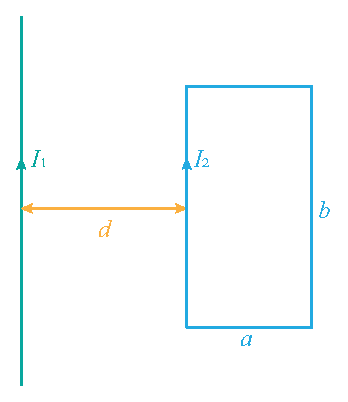
\includegraphics[scale=1.0]{C9-fig5.eps}
	\end{figure}
	
	\begin{solution}
		
		(1) 先求长直导线与矩形线圈间的互感系数M. 假如矩形线框不通电, 而在长直导线中通以向上的电流$I_1$, 则空间的磁场分布为
		
		\begin{equation*}
			B = \dfrac{\mu_0 I_1}{2 \pi r}
		\end{equation*}
		
		穿过矩形线圈的磁通量为
		
		\begin{equation*}
		    \varPhi = N \int \va*{B}_1 \cdot \dd{\va*{S}} = \dfrac{\mu_0 I_1 N}{2 \pi} \int_{d}^{d+a} \dfrac{b}{r} \dd{r} = \dfrac{\mu_0 b I_1 N}{2 \pi} \ln \dfrac{d+a}{a}
		\end{equation*}
		
		互感系数
		
		\begin{equation*}
			M = \dfrac{\varPhi}{I_1} = \dfrac{\mu_0 b N}{2 \pi} \ln \dfrac{d+a}{a}
		\end{equation*}
		
		(2) 当矩形线圈通有变化的电流$I$时(此时设顺时针方向为电流正方形, 直导线中的感应电动势以从下向上为正), 长直导线中的感应电动势为
		
		\begin{equation*}
			\mathscr{E} = -M\dv{I}{t} = - \dfrac{\mu_0 b I_0 \omega N}{2 \pi} \ln(\dfrac{d+a}{a}) \cos \omega t
		\end{equation*}
		
	\end{solution}
	
\end{example}

\begin{example}
	有两根长直平行的传输线, 它们的半径都为$r_0$, 两轴线线相距为$d$, 且$r_0 \ll d$, 如图所示. 求长为$l$的这对传输线的自感.
	
	\begin{figure}[H]
		\centering
		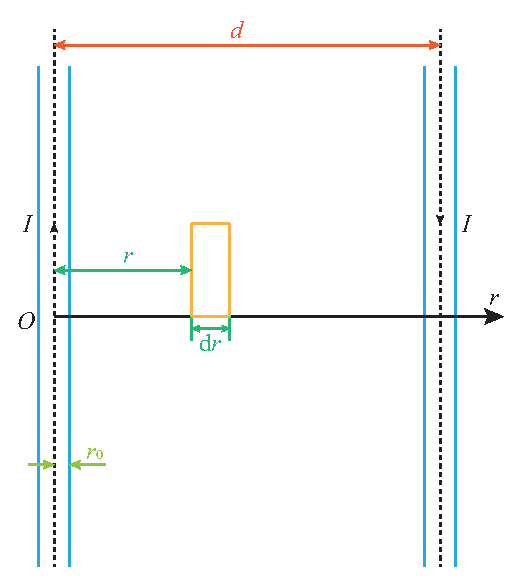
\includegraphics[scale=0.65]{C9-fig6.eps}
	\end{figure}
	
	\begin{solution}
		
		设传输线中通有电流$I$, 通过两传输线间长为$l$, 宽为$d$的面积内的磁通量为
		
		\begin{equation*}
			\varPhi = \varPhi_1 + \varPhi_2
		\end{equation*}
		
		式中$\varPhi_1$, $\varPhi_2$分别为导线1和导线2中电流单独存在时所产生的磁通量. 
		
		由于$r_0 \ll d$, 则可以忽略两导线内部的磁通量. 
		
		导线1在距其轴线$r$处, 宽为$\dd{r}$, 长为$l$的面积元$\dd{S} = l \dd{r}$内产生的磁通量为
		
		\begin{equation*}
			\dd{\varPhi_1} = B_1 \dd{S} = \dfrac{\mu_0 I l}{2 \pi r} \dd{r}
		\end{equation*}
		
		导线1在长为$l$, 宽为$d$的面积内产生的磁通量为
		
		\begin{equation*}
			\varPhi_1 = \int_{r_0}^{d - r_0} \dfrac{\mu_0 I l}{2 \pi} \dfrac{\dd{r}}{r} = \dfrac{\mu_0 I l}{2 \pi} \ln(\dfrac{d-r_0}{r_0})
		\end{equation*}
		
		导线2中的电流与导线1中的电流大小相等方向相反, 所以$\varPhi_1$和$\varPhi_2$量值相等符号相同, 因此
		
		\begin{equation*}
			\varPhi = 2 \varPhi_1 = \dfrac{\mu_0 I l}{\pi} \ln(\dfrac{d-r_0}{r_0})
		\end{equation*}
		
		长为$l$的一对导线的自感
		
		\begin{equation*}
			L = \dfrac{\varPhi}{I} = \dfrac{\mu_0 l}{\pi} \ln(\dfrac{d-r_0}{r_0}) \approx \dfrac{\mu_0 l}{\pi} \ln(\dfrac{d}{r_0})
		\end{equation*}
		
	\end{solution}
	
\end{example}

\section{磁场能量}\label{9.4}

$\bullet$ \textbf{自感磁能}

\begin{equation}
	W_L = \int \dd{W_L} = \int_{0}^{I} L i \dd{i} = \dfrac{1}{2} L I^2 \label{C9-eq18}
\end{equation}

这是通有电流$I$的两个自感线圈$L$中储存的磁能, 又称为自感磁能. 

$\bullet$ \textbf{磁场能量}

在普遍情况下, 磁场中的能量密度可以写成

\begin{equation}
	w_{\textrm{m}} = \dfrac{1}{2} \va*{B} \cdot \va*{H} \label{C9-eq19}
\end{equation}

对于某一空间中磁场的总能量, 它等于$w_{\textrm{m}}$对所占空间的积分

\begin{equation}
	W_{\textrm{m}} = \int_{V} w_{\textrm{m}} \dd{V} = \int_{V} \dfrac{1}{2} \va*{B} \cdot \va*{H} \dd{V}
\end{equation}

\begin{example}
	如图所示, 一同轴电缆由半径为$R_1$的内圆柱导体和半径为$R_2$的圆筒同轴组成, 其间充满了磁导率为$\mu$的磁介质, 内外导体中通有大小相等, 方向相反的轴向电流$I$, 且电流在圆柱体内均匀分布. 求长为$l$的一段电缆内所储存的磁能. 
	
	\begin{figure}[H]
		\centering
		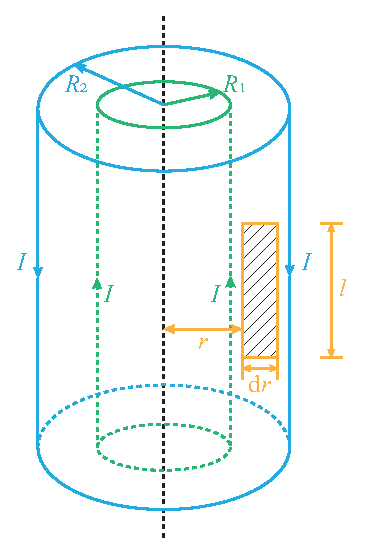
\includegraphics[scale=0.8]{C9-fig7.eps}
	\end{figure}
	
	\begin{solution}
		
		导体整个外表面上为$I$, 内部 + 外部 = $-I+I = 0$, 圆柱体外部无磁场, 而圆柱体内部有磁场. 
		
		长为$l$的一段电缆内所储存的磁能可分为两部分: 一部分是储存在圆柱体与圆筒之间的磁能$W_{\textrm{m}_1}$, 另一部分是储存在圆柱体内部的磁能$W_{\textrm{m}_2}$. 
		
		下面先求$W_{\textrm{m}_1}$. 
		
		根据安培环路定理, 可求得圆柱体与圆筒之间离轴线距离为$r$处的磁感应强度的大小
		
		\begin{equation*}
			B = \dfrac{\mu I}{2 \pi r} \quad \qty(R_1 < r < R_2)
		\end{equation*}
		
		此处的磁能密度为
		
		\begin{equation*}
			w_{\textrm{m}_1} = \dfrac{B^2}{2 \mu} = \dfrac{\mu I^2}{8 \pi^2 r^2}
		\end{equation*}
	
		两导体间磁能密度是$r$的函数, 取半径为$r$, 厚度为$\dd{r}$, 长为$l$的圆柱体外壳体积为$\dd{V}$作为体积元, 则
		
		\begin{equation*}
			\dd{V} = 2 \pi r l \dd{l}
		\end{equation*}
		
		其中磁能为
		
		\begin{equation*}
			\dd{W_{\textrm{m}_1}} = w_{\textrm{m}_1} \dd{V} = \dfrac{\mu I^2}{8 \pi^2 r^2} \cdot 2 \pi r l \dd{l} = \dfrac{\mu I^2 l \dd{r}}{4 \pi r}
		\end{equation*}
		
		储存在长为$l$的内外两载流导体之间的总磁能为
		
		\begin{equation*}
			W_{\textrm{m}_1} = \int_{R_1}^{R_2} \dd{W_{\textrm{m}_1}} = \dfrac{\mu I^2 l}{4 \pi} \int_{R_1}^{R_2} \dfrac{\dd{r}}{r} = \dfrac{\mu I^2 l}{4 \pi} \ln \dfrac{R_2}{R_1}
		\end{equation*}
		
		再求$W_{\textrm{m}_2}$. 
		
		因为内圆柱体横截面内, 电流是均匀分布的, 根据安培环路定理可求得圆柱体内磁感应强度$\va*{B}$的大小为
		
		\begin{equation*}
			B = \dfrac{\mu_0 I r}{2 \pi R_1^2}
		\end{equation*}
		
		因为导体的磁导率接近于真空中磁导率, 故导体中的磁导率取为$\mu_0$, 用上述同样方法可得长为$l$的圆柱导体内储存的磁能为
		
		\begin{equation*}
			W_{\textrm{m}_2} = \int_{V} \dfrac{B^2}{2 \mu_0} \dd{V} = \int_{0}^{R_1} \dfrac{1}{2\mu_0} \qty(\dfrac{\mu_0 I r}{2 \pi R_1^2})^2 \cdot 2 \pi r l \dd{r} = \dfrac{\mu_0 I^2 l}{4 \pi R_1^4} \int_{0}^{R_1} r^3 \dd{r} = \dfrac{\mu_0 I^2 l}{16 \pi}
		\end{equation*}
		
		所以载有电流$I$, 长为$l$的圆柱导体内储存的磁能为
		
		\begin{equation*}
			W_{\textrm{m}} = W_{\textrm{m}_1} + W_{\textrm{m}_2} = \dfrac{\mu I^2 l}{4 \pi} \ln \dfrac{R_2}{R_1} + \dfrac{\mu_0 I^2 l}{16 \pi}
		\end{equation*}
		
		需要指出, 若已知$W_{\textrm{m}}$, 则由
		
		\begin{equation*}
			W_{\textrm{m}} = \dfrac{1}{2} L I^2
		\end{equation*}
		
		可求出自感$L$. 此处长为$l$的同轴电缆的自感$L$为
		
		\begin{equation*}
			L = \dfrac{2 W_{\textrm{m}}}{I^2} = \dfrac{\mu I^2 l}{2 \pi} \ln \dfrac{R_2}{R_1} + \dfrac{\mu_0 I^2 l}{8 \pi}
		\end{equation*}
		
	\end{solution}
	
\end{example}

\section{位移电流}\label{9.5}

把变化的电场也看作是一种电流, 并认为它与传导电流一样能产生磁场, 这种与电位移通量变化有关的电流

\begin{equation}
	I_d = \dv{\varPhi}{t} = \int_{S} \pdv{\va*{D}}{t} \cdot \dd{\va*{S}} = \int_{S} \va*{j}_d \cdot \dd{\va*{S}} \label{C9-eq20}
\end{equation}

称为位移电流, 即通过某曲面的位移电流等于通过该曲面的电位移通量对时间的变化率. 

位移电流密度为

\begin{equation*}
	\va*{j}_d = \pdv{\va*{D}}{t}
\end{equation*}

下面对位移电流的性质作一些说明. 

\begin{enumerate}[itemindent=1em]
	\item 位移电流是电位移通量的变化率, 与传导电流有着本质上的不同. 
	\item 当空间中有介质时, 有
	
	\begin{equation}
		\va*{D} = \varepsilon_0 \va*{E} + \va*{P} \label{C9-eq21}
	\end{equation}
	
	进一步可得
	
	\begin{equation}
		\va*{j}_d = \pdv{\va*{D}}{t} = \varepsilon_0 \pdv{\va*{E}}{t} + \pdv{\va*{P}}{t} \label{C9-eq22}
	\end{equation}
	
	\item 对于接在电路中的导体, 在电流不恒定时, 不仅有传导电流还有位移电流, 但位移电流比传导电流小很多. 
\end{enumerate}


$\bullet$ \textbf{全电流、全电流定理}

\begin{definition}[全电流]
	一般情形下, 通过空间某截面的电流应包括传导电流和位移电流, 它们的代数和称为全电流. 
\end{definition}

\begin{theorem}[全电流定理]
	麦克斯韦将安培环路定理推广为
	
	\begin{equation}
		\oint_{L} \va*{H} \cdot \dd{\va*{l}} = I_s = I_c + I_d \text{~或~} \oint_{L} \va*{H} \cdot \dd{\va*{l}} = I_c + \int_{S} \pdv{\va*{D}}{t} \cdot \dd{\va*{S}} \label{C9-eq23}
	\end{equation}
	
	$I_s$, $I_c$和$I_d$分别代表通过以L为边线的某曲面上的全电流, 传导电流和位移电流. 
\end{theorem}

对于

\begin{equation*}
	\oint_{L} \va*{H} \cdot \dd{\va*{l}} = I_c + \int_{S} \pdv{\va*{D}}{t} \cdot \dd{\va*{S}}
\end{equation*}

若电流连续分布, 则

\begin{equation*}
	I_c = \int_{S} \va*{j}_c \cdot \dd{\va*{S}}
\end{equation*}

其中, $\va*{j}_c$为传导电流密度. 

若传导电流$I_c = 0$, 此时磁场仅由位移电流产生

\begin{equation*}
	\oint_{L} \va*{H} \cdot \dd{\va*{l}} = \int_{S} \pdv{\va*{D}}{t} \cdot \dd{\va*{S}}
\end{equation*}

变化电场同产生的磁场之间呈右螺旋关系, 而变化磁场同感应电场之间呈左螺旋关系. 

\section{麦克斯韦方程组}\label{9.6}

\subsection{静电场与恒定磁场基本规律的回顾}

\begin{enumerate}[itemindent=1em]
	\item 静电场的高斯定理
	
	\begin{equation*}
		\oint_{S} \va*{D} \cdot \dd{\va*{S}} = \int_{V} \rho \dd{V}
	\end{equation*}
	
	反映静电场是有源场, 电荷是产生电场的源. 
	
	\item 静电场的环路定理
	
	\begin{equation*}
		\oint_{L} \va*{E} \cdot \dd{\va*{l}} = 0
	\end{equation*}
	
	反映静电场是有势场, 保守力场或无旋场. 
	
	\item 恒定磁场的高斯定理
	
	\begin{equation*}
		\oint_{S} \va*{B} \cdot \dd{\va*{S}} = 0
	\end{equation*}
	
	反映恒定磁场为无源场. 
	
	\item 恒定磁场的安培环路定理
	
	\begin{equation*}
		\oint_{L} \va*{H} \cdot \dd{\va*{l}} = \sum\limits_{L\text{内}} I
	\end{equation*}
	
	反映恒定磁场是有旋场, 非保守场或涡旋场. 
	
\end{enumerate}

\subsection{麦克斯韦方程组}

麦克斯韦方程组的积分形式: 

\begin{equation}
	\begin{split}
		&\oint_{S} \va*{D} \cdot \dd{\va*{S}} = \sum\limits_{S\text{内}} q_i = \int_{V} \rho \dd{V} \\
		&\oint_{L} \va*{E} \cdot \dd{\va*{l}} = - \int_{S} \pdv{\va*{B}}{t} \cdot \dd{\va*{S}} \\
		&\oint_{S} \va*{B} \cdot \dd{\va*{S}} = 0 \\
		&\oint_{L} \va*{H} \cdot \dd{\va*{l}} = I_s = \int_{S} \qty(\va*{j}_c + \pdv{\va*{D}}{t}) \cdot \dd{\va*{S}}
	\end{split}
    \label{C9-eq24}
\end{equation}

\newpage

麦克斯韦方程组的微分形式: 

\begin{equation}
	\begin{split}
		&\nabla \cdot \va*{D} = \rho \\
		&\nabla \cdot \va*{B} = 0 \\
		&\nabla \times \va*{E} = -\pdv{\va*{B}}{t} \\
		&\nabla \times \va*{H} = \va*{j}_c + \pdv{\va*{D}}{t}
	\end{split}
    \label{C9-eq25}
\end{equation}

利用麦克斯韦方程组的微分形式, 再结合下列介质性能方程

\begin{equation}
	\begin{split}
		&\va*{D} = \varepsilon_0 \varepsilon_r \va*{E} \\
		&\va*{B} = \mu_0 \mu_r \va*{H} \\
		&\va*{j}_c = r \va*{E}
	\end{split}
    \label{C9-eq26}
\end{equation}

共七个方程, 构成了一完整的说明电磁场性质的方程组. 
